\label{chapter:campusstoragepolicylanguage}

\section{Introduction}

In the previous chapter, the HTCondor CacheD was introduced and benchmarked.  In this section, we will discuss the policy framework that allows the CacheD to represent heterogeneous resources on campus or cyberinfrastructure resources.  The CacheD's policy framework is used whenever it interacts with another CacheD.  This policy framework allows the CacheD to act as an independent agent within the distributed system.

In a distributed computing system, independent agents are designed to act on behalf of entities such as users, hosts, or entire clusters.  The agents attempt to fulfill the goals of the entities that they represent, even in the chaotic environment characteristic of a distributed computing system.  In order to fulfill these goals, the agents must know and understand them.  Therefore, a policy language exists to express the goals of the entity.

The policy language must be flexible enough in order to express and follow the goals and instructions of the users.  The goals of the policy language are:

\begin{enumerate}
	\item To express attributes of the entities such as the cache, CacheDs, and the host.
	\item To write policies, taking into account the attributes of the entities.
	\item To be easy to read and write the expressions.
	\item To Allow users to define their semantics and attributes in a schema-free manner.
\end{enumerate}



We implement this policy language in the CacheD using HTCondor ClassAds \cite{raman1998matchmaking}.  ClassAds are an independent library developed by the HTCondor project and are used for communication between HTCondor components.  They provide all of the attributes described above.

\begin{enumerate}
	\item The Key-Value structure of ClassAds allow for attributes of the entities to be expressed in strings, values, lists of string, or expressions.
	\item Expressions can reference attributes in the current and the matching ClassAds.
	\item Expressions are written as expressions with semantics familiar to most programmers.
\end{enumerate}

The CacheD has a few interaction points when it must interact with other agents, such as other CacheDs or users.  Those interaction points are:
\begin{description}
	\item[Choosing a Replication Target] - A CacheD that is the origin to a cache may choose to proactively replicate to other CacheDs.  Choosing a replication target requires matching the cache's requirements with that of the target CacheD's.
	\item[Accepting Cache Replication] - A CacheD must decide if it can accept a cache when it receives a replication request.  This decision is based on its own policy, as well as attributes of the incoming cache.
	\item[Transfer Method] - The transfer method for a cache to be replicated is chosen after a cache has been accepted.  This is a prioritized list of acceptable transfer methods for the cache.

\end{description}



\section{Policy Language}
The policy language used by the CacheD is the HTCondor ClassAds \cite{raman1998matchmaking}.  ClassAds offer the flexibility to describe resources with attributes. 

% example CacheD ClassAd
\begin{figure}
\begin{lstlisting}
CachedServer = true
Machine = "red-foreman.unl.edu"
LastHeardFrom = 1433790880
UpdatesTotal = 8660
Name = "cached-22815@red-foreman.unl.edu"
CondorPlatform = "$CondorPlatform: X86_64-ScientificLinux_6.5 $"
UpdatesHistory = "0x00000000000000000000000000000000"
UpdatesLost = 0
TotalDisk = 6769920
UpdateSequenceNumber = 32307
UpdatesSequenced = 8659
MyAddress = "<129.93.239.170:11000?noUDP&sock=22815_fb39>"
AuthenticatedIdentity = "dweitzel@unl.edu"
DetectedMemory = 7807
Requirements = MY.TotalDisk > TARGET.DiskUsage
CondorVersion = "$CondorVersion: 8.3.1 Dec 22 2014 BuildID: UW_development PRE-RELEASE-UWCS $"
DetectedCpus = 2
DaemonStartTime = 1431839398
CurrentTime = time()
MyCurrentTime = 1433790880
\end{lstlisting}
\caption{CacheD ClassAd Example}
\label{lst:cachedclassad}
\end{figure}

Figure \ref{lst:cachedclassad} shows an example of a CacheD's ClassAd.  The attributes describe the CacheD daemon and the host it runs on.  For example, the \texttt{DaemonStartTime} is a representation of when the daemon started.  \texttt{TotalDisk} describes how much disk is available on the host where the CacheD is running.

% How matching works
Matching of ClassAds is done by comparing attributes between two sets of ClassAds.  The attribute \texttt{Requirements} takes a special meaning when matching two ClassAds.  The 
\texttt{Requirements} attribute is a boolean expression that is evaluated in the context of both the current ClassAd and the matching ClassAd.  In the example in Figure \ref{lst:cachedclassad}, the CacheD's ClassAd would only match another ClassAd if the expression is \texttt{MY.TotalDisk > TARGET.DiskUsage}.  This means that the CacheD will only accept caches that are smaller in size than the available disk on the host.  \texttt{MY} and \texttt{TARGET} refer to the current ClassAd and the matching ClassAd, respectively.


The \texttt{Requirements} attribute in Figure \ref{lst:cachedclassad} references other attributes in both the current ClassAd and the matching ClassAd.  Attributes can reference other attributes in order to form strings, lists, or boolean expressions.  In this example, the \texttt{Requirements} attribute references other attributes in order to create a boolean expression.

\begin{figure}[h!t]
	\centering
	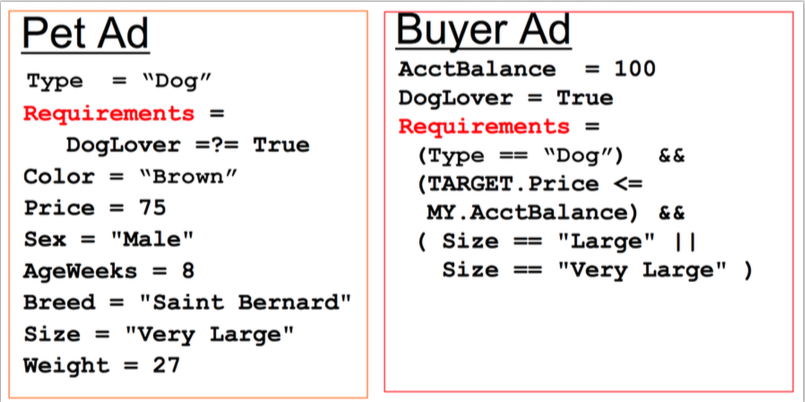
\includegraphics[width=0.8\textwidth]{images/ClassAdExample.png}
	\caption{ClassAd Example Showing Usage of Requirements}
	\label{fig:classadexample}
\end{figure}

An example of using the \texttt{Requirements} attribute is shown in Figure \ref{fig:classadexample}.  In this example, we have two ads.  A pet which describes the attributes of a dog and a buyer ad which describes the attributes of a potential buyer.  The pet ad has the requirements that the buyer is a \texttt{DogLover}.  The buyer has the requirements:

\begin{itemize}
	\item The pet must be a dog.
	\item The pet must cost less than the money the buyer has.
	\item The pet must be ``Large'' or ``Very Large''.
\end{itemize}

In the example, the pet ad would match the buyer ad.

\subsection{Extending CacheD Attributes}

% Extending policy language
The ClassAd describing the CacheD can be extended by using the CacheD Cron mechanism.  The CacheD Cron executes an external program in order to collect statistics and report the results in the CacheD's ClassAd.  These statistics can then be used to better describe either the daemon or the host machine.  The CacheD Cron is configured by specifying the job's attributes in the HTCondor configuration.

\begin{figure}[h!t]
\begin{lstlisting}
CACHED_CRON_CONFIG_VAL = $(RELEASE_DIR)/bin/condor_config_val
CACHED_CRON_JOBLIST = $(STARTD_CRON_JOBLIST) test
CACHED_CRON_TEST_MODE = Periodic
CACHED_CRON_TEST_EXECUTABLE = $(RELEASE_DIR)/test.sh
CACHED_CRON_TEST_PERIOD = 15s
\end{lstlisting}
\caption{CacheD Cron Configuration}
\label{lst:cachedcronconfiguration}
\end{figure}

Figure \ref{lst:cachedcronconfiguration} shows the configuration in order for the CacheD to periodically run a program named ``test.''  The executable, \texttt{test.sh}, will run tests and output a ClassAd that will be merged into the CacheD's ClassAd.  It will be run  at periods of every 15 seconds.


\begin{figure}
\begin{lstlisting}
TestResult = 100
TestRan = TRUE
TestHost = "hostname.unl.edu"
\end{lstlisting}
\caption{Example Output from CacheD Cron: \texttt{test.sh}}
\label{lst:cachedcronoutput}
\end{figure}

The output of the test executable is ClassAds that will be injected into the daemon.  Figure \ref{lst:cachedcronoutput} shows the example output from running the test program.  In this output, it sets three attributes, an integer, a boolean value, and a string.  

A example of using the CacheD Cron is to measure the IO operations per second that a host is able to complete.  This information can be used to better match caches with machines which can run the applications.  
%The period of testing the IO capabilities of a node should be longer than the 15 seconds shown in Figure \ref{lst:cachedcronconfiguration}.


\section{Uses of the Policy Language in the CacheD}

The CacheD uses the ClassAd policy language when communicating with other daemons.  For each interaction, the CacheD must make a decision, and therefore relies on the ClassAd policies in order to decide whether to perform an action.  Each of these actions are described briefly in the introduction to this chapter.  We will now discuss the details of those interactions and choices the CacheD may make in the next few sections.


\subsection{Choosing a Replication Target}
% when it is used, and by who
Each cache has a single ``origin CacheD.''  This CacheD is the CacheD where the user initially uploaded the cache.  This origin CacheD has the option to proactively replicate the cache without it being requested by jobs.  The data transfer can occur while another job is currently being run.

% What is it matching against
The origin CacheD will periodically query the HTCondor Collector to receive a list of CacheD ClassAds.  Then, the origin will iterate through each of these ClassAds, attempting to match the cache with a CacheD.

For each ClassAd from the cache and a remote CacheD, the origin will attempt a mutual match.  Therefore, the cache must accept the CacheD, and the CacheD must accept the cache.  The \texttt{Requirements} expression is evaluated for both of the ClassAds.  The default basic \texttt{Requirements} expression is to require that the CacheD has enough disk space for the cache.

For the CacheD, the default \texttt{Requirements} are:
\begin{lstlisting}
Requirements = MY.TotalDisk > TARGET.DiskUsage
\end{lstlisting}

And for an uploaded cache, the default \texttt{Requirements} are:
\begin{lstlisting}
Requirements = MY.DiskUsage < TARGET.TotalDisk
\end{lstlisting}

\texttt{MY} refers to attributes in the current ClassAd, while \texttt{TARGET} refers to attributes in the matching ClassAd.  \texttt{TotalDisk} is the amount of disk available to a CacheD.  \texttt{DiskUsage} is the total file size of the cache.  An example value of the \texttt{TotalDisk} can be seen in the example ClassAd of a CacheD shown above in Figure \ref{lst:cachedclassad} on page \pageref{lst:cachedclassad}.

% What if it does match

If the cache and remote CacheD match, the origin CacheD will send a cache replication request to the remote CacheD.  The remote CacheD will then decide if it will accept the replication request.

% What if it does not match
If the two do not match, then the origin server will not send a replication request to the remote CacheD.

% Special attributes
Additionally, there are special attributes available during this matching.  One special attribute used during some of the experiments is the \texttt{CacheRequested} attribute.  This attribute is set to the boolean \texttt{TRUE} when the cache is requested by a job.  When the cache is requested by a origin CacheD replication request, it is set to \texttt{FALSE}.  This attribute can be used in a cache's \texttt{Requirements} expression to limit cache replication to only those nodes that have jobs that have requested the cache.  An example expression would be:
\begin{lstlisting}
Requirements = (MY.DiskUsage < TARGET.TotalDisk) && (TARGET.CacheRequested =?= true)
\end{lstlisting}

Further special attributes are planned, such as an attribute whose value is the number of replications of the cache already completed.  This can be used to limit the number of CacheDs that have the cache.

\begin{table}[h!t]
	\centering
	\bgroup
	\def\arraystretch{1.5}
\begin{tabular}{l | p{10cm}}
\textbf{Attribute} & \textbf{Use} \\ \hline
\texttt{CacheRequested} & Boolean cache property set to \texttt{TRUE} when the cache has been requested by a job. \\
\texttt{CacheReplicas} & Cache property available on the cache origin.  A numerical value representing the number of complete replicas stored by CacheDs. \\
\texttt{DiskUsage} & Size, in kilobytes, of the cache. \\
\texttt{TotalDisk} & Available disk, in kilobytes, to store caches. \\
\texttt{BandwidthUsed} & Bandwidth used on the CacheD host, in Gbps. \\
\texttt{CacheDIops} & CacheD property of current measured IOPS on the host. \\
\texttt{ActiveTransfers} & Number of active transfers on the CacheD.
\end{tabular}	
	\egroup
	\caption{Sample CacheD Attributes}
	\label{tbl:cachedattributes}
\end{table}

\subsection{Accepting Cache Replication}
% When it is used, and by who
A CacheD can receive cache replication requests from three sources:

\begin{enumerate}
	\item An origin CacheD sending out proactive replication requests.
	\item A job requesting a cache.
	\item A child CacheD (as described in section \ref{sec:cachedparenting}).
\end{enumerate}

In each of these requests, the receiving CacheD has the choice to accept the replication or deny it.  When it receives a cache replication request, it looks up the cache's ClassAd and does mutual matching with its own ClassAd.  This is similar to the mutual matching done when an origin CacheD is issuing proactive replication requests.  It is important to re-run this mutual matching in case the CacheD's state has changed.  The CacheD's state could change if it has downloaded a large cache, therefore, altering the available disk for additional caches.

If the CacheD's mutual matching with the cache's ClassAd is successful, then the CacheD will accept the cache and begin negotiating transfer methods.  If the CacheD and the cache's ClassAd do not match, then the CacheD will reject the cache.

The approval or rejection of the cache is done asynchronously from the request for replication.  Therefore, the CacheD keeps a data structure of rejected caches (accepted caches are kept in the local cache database).  When the client next asks for the replication status of the cache, the CacheD will respond with the accept or reject status.  The cached rejection request expires after 15 minutes.


\subsection{Transfer Method}

% Who uses it
Each cache has a list of acceptable transfer methods.  A user may set this list of acceptable transfer methods when uploading the cache.  This list is priority ordered, with the preferred transfer method listed first.

% List formation
\begin{figure}
\begin{lstlisting}
ReplicationMethods = "BITTORRENT, DIRECT"
\end{lstlisting}
\caption{Example Replication Method for a Cache}
\label{lst:cachetransferlist}
\end{figure}

In the example shown in Figure \ref{lst:cachetransferlist}, the cache has a preference for transferring the files over BitTorrent, but will accept the Direct transfer method if needed.  Transfer methods are described in full in Section \ref{sec:cachedtransfermethods}.  These are the only possible methods now, but may expand to other methods in the future.

% Negotiating preferences
After accepting a cache to be downloaded, the CacheD will negotiate the transfer method with the cache's ClassAd that was downloaded during the acceptance testing stage. The cache's ClassAd includes the \texttt{ReplicationMethods} attribute, which is a priority list of acceptable transfer methods.  The CacheD has its own \texttt{ReplicationMethods} that is set in its configuration.  The CacheD iterates through its own methods until it finds a matching transfer method in the cache's methods.

As an independent agent, the CacheD prefers its own transfer priority list rather than the cache's priority list.  Psuedo code for the transfer negotiation is shown in Algorithm \ref{alg:negotiatetransfer}.

\begin{algorithm}
\caption{Negotiating Transfer Method Function}
\begin{algorithmic}
\State $cacheMethods\gets cacheClassAd[ReplicationMethods]$
\State $cachedMethods\gets config(ReplicationMethods)$
\ForAll{$cachedMethod \in cachedMethods$}

\ForAll{$cacheMethod \in cacheMethods$}
\If{$cachedMethod = cacheMethod$} 
\State \Return $cachedMethod$
\EndIf


\EndFor

\EndFor
\end{algorithmic}
\label{alg:negotiatetransfer}
\end{algorithm}
	
	

%\section{Inserting Attributes into Policy}

%\subsection{Measuring Storage}
%In order to provide matchmaking for resources, the resources need to be accurately described and advertised.  This requires measuring the storage capabilities and capacity of the resources and advertising those attributes to the catalog of resources.

%The measurements must be performed on the execution targets as they are the temporary storage targets.  The execution targets will measure the storage capabilities in order to determine if the jobs can run.

%TODO: Talk about measuring storage values

\section{Example Policies}

In order to better describe how data should be moved, we must categorize the data as shared or unique, private or non-private.  This creates a 2x2 matrix of possibilities of data.  Below, we define each of these categorizations.  Each of these categories comes with its own restrictions on how the data may be moved and how it is presented to the user.

\begin{table}[h!t]
	\bgroup
	\def\arraystretch{1.5}
\begin{tabular}{l | l | l }
& \textbf{Public} & \textbf{Private} \\ 
\hline
\textbf{Shared} & Executables and Libraries & Personal Identifying Information \\ 
\hline
\textbf{Unique} & Input Parameters & BLAST Query Files \\
\hline
\end{tabular}
\egroup
\caption{Example Data Types}
\label{tbl:exampledatatypes}
\end{table}

Shared data is data that is the same for multiple jobs in a job set.   In many cases, the majority of the files in the job sandbox can be considered shared data.  Examples of shared data are job executables and libraries.  

Frequently the job executables are the same for a large number of jobs.  Since the executables are the same, contextualization of the job is done through other methods, such as arguments or parameter files.  An example application that would use the same executables and libraries are Monte Carlo \cite{binder2010monte} simulations.  In these applications, the executables are the same for every job.  Each job is given a unique identifier which is used for the starting condition for the random generation.

Experimental data could also be shared between multiple jobs in a job set.  This can include common input data such as databases.  For example, BLAST \cite{altschul1990basic} jobs require a database of sequences of proteins which are then matched with specific queries.  The database is typically the same for a large number of queries.  

We define unique data as data which is different for each job.  The unique data may be small, such as parameter files.  Or they may be large, such as sections of a database to search.  By definition, unique data is defined as data which would not benefit from shared transfer; no other job needs the same data.

For our consideration, data which is not the same for every job in a job set, but is shared between jobs in a subset of the jobs, will be considered shared data.

% private versions of shared and unique
We define private data as data which the user wants to prevent others from viewing.  The level of privacy requested by a user could determine how it can be enforced.  It could be enforced through authenticated access, encrypted data transfers, or both.  In most cases, authenticated data access is sufficient.

Private versions of shared and unique data cannot use the same optimization as public data.  For example, the data could not be transferred using a caching daemon if authenticated access is required.   Transferring data unauthenticated, even encrypted, is dangerous due to susceptibility to brute force decryption.



An example policy for a cache that is composed of public shared data could be:

\begin{lstlisting}
Requirements = MY.DiskUsage < TARGET.TotalDisk
ReplicationMethods = "BITTORRENT, DIRECT"
\end{lstlisting}

This policy will allow the CacheD to proactively replicate the caches to available CacheDs.  Further, it will allow the CacheD to replicate using the BitTorrent method, or the Direct method if the remote CacheD does not support or prefer BitTorrent.  

For private shared data, an example policy would look like:

\begin{lstlisting}
Requirements = (MY.DiskUsage < TARGET.TotalDisk) && (TARGET.CacheRequested =?= true)
ReplicationMethods = "DIRECT"
\end{lstlisting}

In this method, the cache would only be replicated to nodes where it is requested.  This will minimize the number of nodes that have this private data stored.  Second, it will use the \texttt{DIRECT} method of distribution, which uses an authenticated and optionally encrypted method of transfer.  

Unique data cannot benefit from caching.  But it can benefit from faster transfers.  As we have seen in Chapter \ref{chapter:campusdatadistribution}, even when caching is not turned on, the unique transfer methods that the CacheD uses can benefit the stage-in time for this unique data.  It is possible to package many jobs worth of unique data into a cache and transfer the cache for each job.  Then, on subsequent execution that require unique data from the package, it will be immediately available from the CacheD's cache.

Packaged unique private data can be transferred with the same policies as shared private data.  Unique public data can be transferred with shared public policies.

\subsection{Policies Utilizing Extended Attributes}

Since ClassAds are schema-less and extendable, attributes can be added that can help in matching.

One example policy is to ban BitTorrent at certain OSG sites.  This policy is useful if sites have policies against certain transfer methods.  While running our experiments from the previous chapter, we were contacted by the administrators of the clusters at Brookhaven National Lab (BNL).  They discovered that we were running BitTorrent on their clusters, contrary to their policy.  The following policy would only use the Direct transfer method at BNL.

\begin{lstlisting}
Requirements = (MY.DiskUsage < TARGET.TotalDisk) && (TARGET.CacheRequested =?= true)
ReplicationMethods = ifThenElse(regexp(".*.bnl.gov$", TARGET.Name), "DIRECT", "BITTORRENT,DIRECT")
\end{lstlisting}

The \texttt{Requirements} are similar to previous policies.  The \texttt{ReplicationMethods} uses the \texttt{ifThenElse} ClassAd function in order determine which replication method to use.  It uses a regular expression to determine if the target CacheD is from BNL.  It tests if the \texttt{Name} ends with the domain name of the \texttt{bnl.edu}, the domain for BNL.  If it does match, then the Direct method is chosen.  If the \texttt{Name} does not match \texttt{bnl.edu}, then both BitTorrent and Direct methods are allowed.

Administrators can add custom attributes using the CacheD Cron.  For example, administrators could add attributes that list the organizations that own the storage resources.  When this attribute is available, both the CacheD and the caches can make policies that will use it.

An example CacheD policy:
\begin{lstlisting}
CacheDOwners = "CMS,HCC"
Requirements = (MY.TotalDisk > TARGET.DiskUsage) && stringListIMember(TARGET.CacheOwner, MY.CacheDOwners)
ReplicationMethods = "BITTORRENT,DIRECT"
\end{lstlisting}

In this policy, the CacheD would only accept replications of caches which have the attribute \texttt{CacheDOwners} and it is set to either \texttt{CMS} or \texttt{HCC}.  There is no method of enforcing the requirement that only members of the CMS or HCC organizations have this have this attribute; therefore, you must create a trust relationship with CacheDs that are allowed to communicate.

A cache policy that would match this policy is:
\begin{lstlisting}
CacheOwner = "HCC"
Requirements = (MY.DiskUsage < TARGET.TotalDisk)
ReplicationMethods = "BITTORRENT,DIRECT"
\end{lstlisting}

Further, a cache could set a policy to only replicate to resources that are owned by the same organization that they belong:
\begin{lstlisting}
CacheOwner = "HCC"
Requirements = (MY.DiskUsage < TARGET.TotalDisk) && stringListIMember(MY.CacheOwner, TARGET.CacheDOwners)
ReplicationMethods = "BITTORRENT,DIRECT"
\end{lstlisting}



%\subsection{Ranking Storage}
%In order to find the most ideal resource for a job, the resources need to be ranked.  The simplest is a greedy approach where the resources are simply ranked by their benchmark speeds.  Additionally, they should only be ranked on the attributes requested by the job, i.e. if the job is only requesting X iops, then only rank resources on the IOPS available.

%It is not immediately clear how the ranking should work.  If we assume that the user accurately describes their application needs, then we can pack the jobs onto resources by placing the job on the resource that meets the IOPS requirements, but has the least amount of IOPS remaining.  This will be an area of research to compare scheduling techniques on execution resources when considering their storage capabilities.


%\section{Data Movement}
%We will consider three different types of data.  The input data, output data, and the job sandbox.  The job sandbox is the environment from which the job will run.  The sandbox is important since the user designs their job to run in this sandbox, and it must be maintained in order for the job to run.  Also, the sandbox is shared input data that multiple executions of the job can utilize.

%The sandbox is a set of files that must be present when the job begins execution.  For example, a sandbox may contain:
%\begin{itemize}
%\item The executable that the job will run.
%\item Libraries necessary for the executable to properly function.
%\item Shared input files such as parameter files or calibration data.
%\end{itemize}

%Some input data could be unique per job, therefore will be considered separately from the job sandbox.  Shared data between many executions can benefit from caching, where unique input data cannot benefit from caching.

%Data for each job can be categorized as either shared, unique, private shared, or private unique.

%\subsection{Categorizing Data}
% Describe shared data



 

% May go into introduction
%Many optimizations may be done to transfer shared data.  For example, people have used caching \cite{blumenfeld2008cms} the shared data per site.  Others have experimented using group transfer protocols such as Bittorrent \cite{cohen2008bittorrent} to distribute the shared data \cite{wei2005collaborative}.

% unique data



%After finding a resource to run on, the job sandbox and input data must be transferred to the remote host.  In order to do this, the remote execution host and the submitter must negotiate how to get the data there.  For example, does the remote host have access to the same NFS server?  Can it mount it?

%\section{Description for these items}
%Logically, we can separate these items into 2 categories
%\begin{itemize}
%\item Requirements for the application
%\item Acceptable methods of data movement
%\end{itemize}

%The users must specify these items in the description of their jobs.  No consensus language for these specifications currently exists.  

%The language for the requirements will be similar to the current specifications for memory and cpu.  The user will request certain storage parameters, and machines will need to provide these metrics just as they do now with cpu and memory.

%The acceptable methods for data movement can either be specified by the user, or by the submitting system.  The system can stage the data to a third party, which will then be used for the transfer to the execution target.  This can be especially useful if multiple jobs use the same input data, a useful example of this is HCC�s use of LVS \cite{zhang2000linux} to serve common files on the OSG.  The server could automatically choose to use HTTP to transfer the files, especially since there are many common files, and the files would be cached on the remote sites using normal HTTP proxy caches.

%Another possible scenario is when starting a job on Amazon EC2.  If it is a virtual machine job, then input data could be created as a CD drive, or a block device, and input into the machine using the block device as input storage.

%\section{Policy language for matchmaking storage}
%The goal is to enable the user to describe their application to the scheduler in such a way that the scheduler can make intelligent decisions on:
%\begin{itemize}
%\item If the application can run on the pool
%\item Where is the ideal location for the job to run
%\item How to get the data to and from the application
%\end{itemize}

% An example policy language for a job is:

\section{User Scenario}
%TODO: work on user scenario

In order to illustrate a user's experience with the policy language, we will use the BLAST example that is used in the previous chapter's experiments.  In this example, we have three types of data:

\begin{description}
	\item[BLAST Database:] A shared public database which will be used by every execution of the job.  The database is widely distributed; therefore, there is no private data to hide.
	\item[BLAST Executables:] Public executables that are originally from the NIH website.  They will be used by every job in the workflow.
	\item[Query Files:] Multiple small files that may not be public.  Each query file is used only by one job.
\end{description}

The BLAST database was shown to be optimally distributed in Chapter \ref{chapter:campusdatadistribution} with the CacheD and BitTorrent.  Therefore, the user would first create the cache, then give it the policy to be proactively replicated to caches with BitTorrent.

\pagebreak

\begin{lstlisting}
$ importCache nrdb <path/to/db>/nrdb*
$ setReplicationPolicy "MY.DiskUsage < TARGET.TotalDisk" "BITTORRENT,DIRECT"
\end{lstlisting}


Next, the BLAST executables are much smaller than the BLAST database, but they are used by every execution.  Therefore, they would benefit from caching and we will use the CacheD.  Since executables are small, the replication will not take long, therefore is no need to proactively replicate the executables.  But, there is nothing private in the BLAST executables, therefore they will be distributed over BitTorrent or Direct method.

\begin{lstlisting}
$ importCache blast_executables <path/to/exes>/blast*
$ setReplicationPolicy "(MY.DiskUsage < TARGET.TotalDisk) && (TARGET.CacheRequested =?= true)" "BITTORRENT,DIRECT"
\end{lstlisting}

Finally, the BLAST queries may be private.  The queries are stored in many small files.  The queries may or may not be optimally transfered and managed by the CacheD.  If the BLAST jobs are short, then the submission node could constantly be transferring the query files to resources that need them.  If the number of running jobs is significant, then this could become a bottleneck.  Using the CacheD, the researcher could avoid significant transfers from the submit host.  By grouping all the queries into a single cache, then transferring that cache for each job, any other jobs on that same node would request the file from the cache rather than the submission node.  If the jobs are short, then this cache would be used often, at the cost of transferring all of the queries the first time.

Since the queries are private, the CacheD must transfer them with the Direct method so that the transfers are authenticated and encrypted.  Further, the CacheD must only replicate them to the nodes that actually request them, so as to not expose the queries on more nodes than necessary.

\begin{lstlisting}
$ importCache blast_executables <path/to/exes>/blast*
$ setReplicationPolicy "(MY.DiskUsage < TARGET.TotalDisk) && (TARGET.CacheRequested =?= true)" "DIRECT"
\end{lstlisting}


%A user creates their submit file and specifies their data.  The above policies will be matched to syntax in the submit file.  The syntax is shown in Listing \ref{lst:inputsyntax}.  We illustrate a shared, non-private case using a BLAST database, and a unique private file with the BLAST queries in Listing \ref{lst:blastsyntax}.  

%\begin{figure}[h!]
%\centering
%\begin{lstlisting}[frame=single,caption={Input Syntax},captionpos=b,label={lst:inputsyntax}] 
%{shared|unique}_{public|private}_input = <file1>,<file2>,...
%\end{lstlisting}
%\end{figure}



%\begin{figure}[h!]
%\centering
%\begin{lstlisting}[frame=single,caption={Blast input syntax},captionpos=b,label={lst:blastsyntax}]
%shared_public_input = blast_database.fasta
%unique_private_input = queries
%\end{lstlisting}
%\end{figure}


%The blast database is public, so there is no need to encrypt or authenticate access to the database.  Further, the database is shared between all executions of the job. The \texttt{queries} may contain personal identifiable information, and are therefore private and need authenticated access control in order to access the data.  

%When the job begins, it will be guaranteed to have the files \texttt{blast\_database.fasta} and \texttt{queries} available to it.  The job framework will decide on the method of transfer and transient storage based on negotiation between the user specified syntax, the worker node, and the submit node.


%\section{Defining Storage Target}
%In this section, we define storage based on it�s capabilities:
%\begin{itemize}
%\item The total space available for an application or set of applications to store data.
%\item The bandwidth available to the storage target.
%\item The IOPS available to read / write to the storage (more applicable to local storage).
%\item Access Protocol
%\end{itemize}

%Therefore, when mentioning storage, we must specify or estimate or discover all of these attributes.


\section{Conclusions}

In a distributed computing system, independent agents are designed to act on behalf of entities such as users, hosts, or entire clusters.  A policy language must exist so that the entities can express their goals to the agents.  

In this chapter, we have designed a policy language based on the HTCondor \mbox{ClassAds} that can be used for expressing policy in data distribution.  We have identified three interaction points for caching agents and designed the semantics for their interaction.

Additionally, we described different input data scenarios and possible replication policies for them.  We gave a recommended policy configuration for the popular BLAST application, including explanations on the policy configuration.  We also included the commands to create and set the policy configuration.

The policy language has been implemented in the CacheD, where it has been tested in Chapter \ref{chapter:campusdatadistribution}.  Further, we illustrated a user scenario of setting this policy language.







%\section{Another Method for Data Transfer}
%In addition to the above methods for transferring data to remote worker nodes, and specifying storage parameters, we can also provide another method for getting data to worker nodes that will better fit the current state of clusters and cyberinfrastructure.  The proposed methods is a dynamic deployment of a storage federation.  This can be done across a single cluster, across many clusters, or over an entire national infrastructure such as the OSG.

%This new method for data transfer relies on peer to peer transfers.  Data is transferred from it�s peer rather than from a single host.  As with all peer to peer systems, the benefits from this method include decreasing the required bandwidth from any single source.  As well as lower latency transfers.
